\documentclass[a4paper,12pt]{article} 
\usepackage[T2A]{fontenc}			
\usepackage[utf8]{inputenc}			
\usepackage[english,russian]{babel}	
\usepackage{amsmath,amsfonts,amssymb,amsthm,mathtools} 
\usepackage[colorlinks, linkcolor = blue]{hyperref}
\usepackage{upgreek}
\usepackage[left=2cm,right=2cm,top=2cm,bottom=3cm,bindingoffset=0cm]{geometry}
\usepackage{multirow}
\usepackage{graphicx}
\usepackage{xcolor}
\usepackage{multirow}
\usepackage{pgfplots}
\usepackage{pgfplotstable}
\pgfplotsset{compat=1.9}

\pgfplotstableset{ %
        create on use/SquareLight/.style={
                create col/expr={\thisrow{Dark}}}
}

\author{Шелихов Дмитрий\\Группа Б01-305}

\title{\textbf{Работа 3.6.1\\Cпектральный анализ электрических сигналов}} 
\date{\today}

\begin{document} 

\maketitle

\textbf{Цель работы:} изучить спектральный состав периодических электрических сигналов.
\par
\textbf{В работе используются:} анализатор спектра (аналоговый или цифровой), генератор прямоугольных импульсов и сигналов специальной формы, осциллограф.\\
\noindent\textbf{Теоретическая справка}

Периодическая функция может быть представлена в виде бесконечного ряда гармонических функций - ряда Фурье:

$$ f(t) = \sum\limits_{n=-\infty}^{\infty} c_ne^{in\omega_0t}  $$

$$\omega_0 = 2\pi/T \text{,где T - период функции f(t). Коэффициенты {$c_n$} могут быть найдены по формуле: }$$
$$ c_n = \frac{1}{T}\int_0^Tf(t)e^{-inw_0t}dt. $$

Простейший спектральный анализатор - высокодобротный колебательный контур с подстраиваемой ёмкостью или индуктивностью.

\center{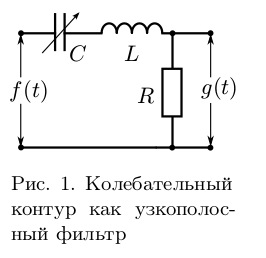
\includegraphics[width=.4\textwidth]{1.png}}

Такой контур усиливает гармоники входного сигнала f(t), частота которых близка к резонансной $\nu_0$ = $\frac{1}{2\pi\sqrt{LC}}$, и практически не реагирует на частоты, далёкие от $\nu_0$. Таким образом, с точки зрения преобразования сигналов, такой контур является является узкополосным фильтром с шириной полосы пропускания порядка $\Delta\nu \approx \nu_0/Q$, где Q = $\frac{1}{R}\sqrt{\frac{L}{C}}$ >> 1 - его добротность.  

При этом амплитуда колебаний в контуре пропорциональна амплитуде |c($\nu_0$)| гармоники в спектре функции f(t), частота которой совпадает с $\nu_0$. Таким образом, меняя резонансную частоту контура, можно просканировать весь спектр входного сигнала. \\

\noindent \textbf{Экспериментальная установка}
	Рассмотрим следующую схему: 	
Исследуемый сигнал f(t) и синусоидальный сигнал от вспомогательного генератора, называемого в таких системах \textbf{гетеродином}, подаются на вход \textbf{смесителя}. Смеситель преобразует колебания с частотами $\nu_1$ и $\nu_2$ в колебания на комбинированных частотах: $\nu1 + \nu2$ и $\nu1 - \nu2$. Сигнал смесителя поступает на фильтр, настроенный на фиксированную резонансную частоту $\nu_0$. То есть, если f(t) содержит гармонику $\nu = \nu_{гет} - \nu_0$, она будет усилена, а отклик будет пропорционален её амплитуде.

\center{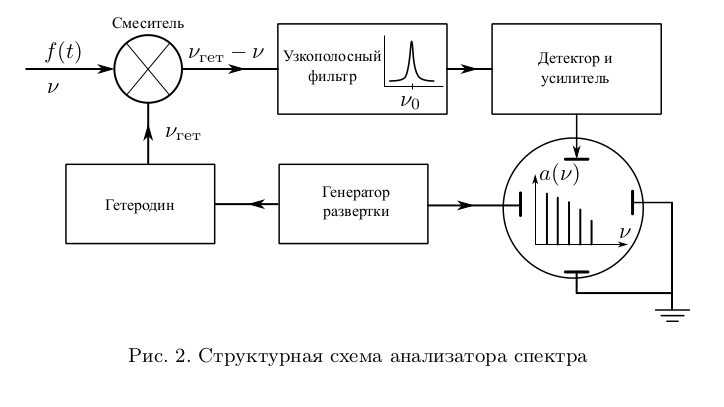
\includegraphics[width = .8\textwidth]{2.png}}

На экране анализатора возникает график, изображающий зависимость амплитуды гармоник исходного сигнала от частоты, т.е. его спектр.\\

\textbf{Ход работы}\\

\textbf{А. Исследование спектра периодической последовательности прямоугольных импульсов}\\

Исследуем зависимость ширины спектра $\Delta\nu$ периодической последовательности прямоугольных импульсов от длительности отдельного импульса $\tau$. 

\noindent 1) Ознакомимся с устройством приборов: генератор прямоугольных импульсов, осциллограф, анализатор спектра и подготовим их к работе, следуя техническим описаниям. 

\center{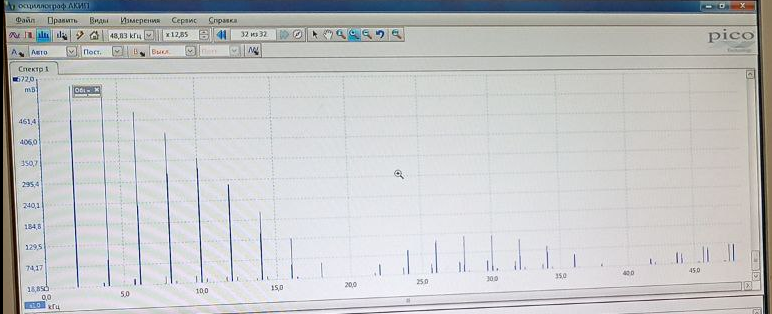
\includegraphics[width=.8\textwidth]{3.png}}

\noindent 2) Подключим генератор прямоугольных импульсов через разветвитель к осциллографу и анализатору спектра.

\noindent 3) На генераторе зададим частоту повторения импульсов $\nu_{\text{повт}}$ = 1кГц (период T = 1мс), длительность импульса $\tau$ = 50 мкс. Получим устойчивую картину сигнала на осциллографе. 

\noindent 4) Предварительно оценим характерную ширину спектра из соотношения неопределённостей $\Delta\nu \approx 1/\tau$ = 20 кГц. 

\noindent 5) Получим спектр сигнала на анализаторе спектра. Предварительно подберём начало отсчёта и диапазон измерения по частоте, так чтобы на экране помещалась большая часть спектра.

\noindent 6) Изменяя параметры сигнала ($\nu_{\text{повт}}$, $\tau$), пронаблюдаем как изменяется его спектр.

\begin{figure}[h]
\center{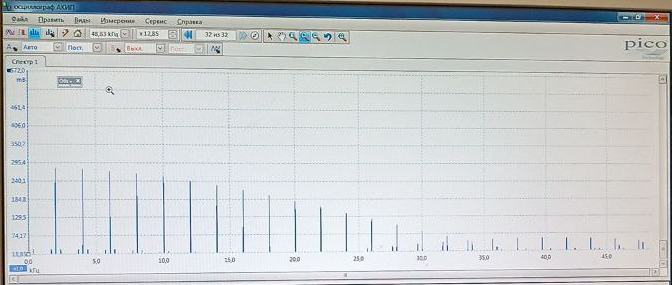
\includegraphics[width=.6\textwidth]{4.png}}
\caption{$\nu_{\text{повт}}$ = 1кГц, $\tau$ = 50мкс}
a) Картинка для сравнения
\end{figure}

\begin{figure}[h]
\center{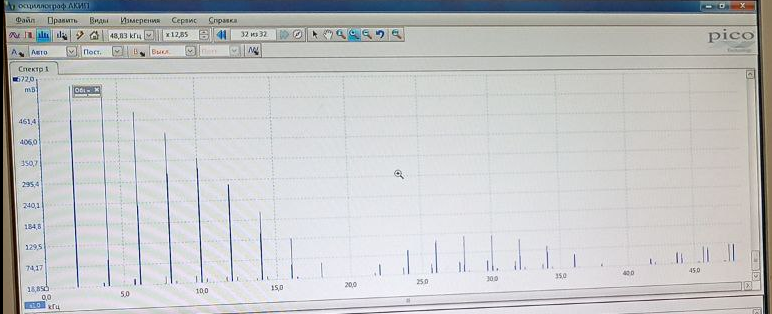
\includegraphics[width=.6\textwidth]{5.png}}
\caption{$\nu_{\text{повт}}$ = 2кГц, $\tau$ = 50мкс}
б) При увеличении $\nu_{\text{повт}}$ амплитуды гармоник увеличиваются, ширина спектра не меняется.
\end{figure}

\begin{figure}[h]
\center{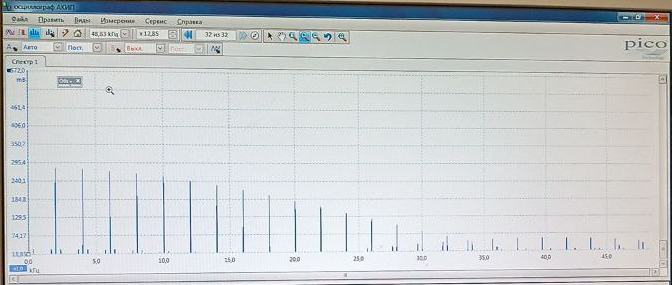
\includegraphics[width=.6\textwidth]{6.png}}
\caption{$\nu_{\text{повт}}$ = 2кГц, $\tau$ = 25мкс}
в) При уменьшении $\tau$ амплитуды уменьшаются, ширина спектра увеличивается.
\end{figure}

\begin{figure}[h]
\center{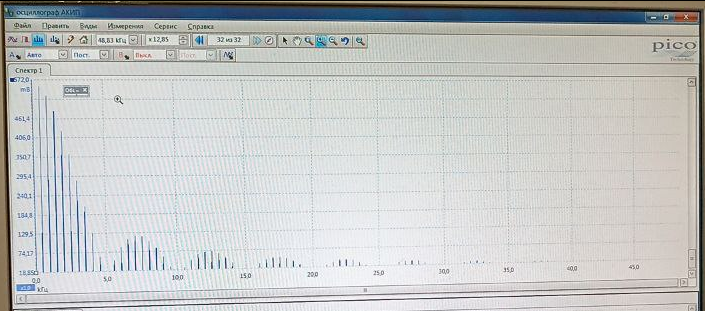
\includegraphics[width=.6\textwidth]{7.png}}
\caption{$\nu_{\text{повт}}$ = 0,5кГц, $\tau$ = 200мкс}
г) Амплитуды возросли, ширина спектра уменьшилась. (в результате суперпозиции пунктов б и в) 
\end{figure}

Масштаб частот по оси X на всех изображениях один и тот же.

\noindent 7) Проведём измерения зависимости ширины спектра от длительности импульса $\Delta\nu$($\tau$) при изменении $\tau$ от 25 до 200 мкс при $\nu_{\text{повт}}$ = 1 кГц. Ширину определяем по положению первой гармоники с нулевой амплитудой.






\end{document}
